\documentclass{beamer}
\usepackage{tikz}
\usetikzlibrary{calc,arrows.meta}
\usepackage{xcolor}
\usepackage{multicol}
\usepackage{amsmath}

\title{Areas, Perimeters \& Averages}
\author{}
\date{}

\begin{document}

\frame{\titlepage}

%------------------------------------------------
% SLIDE 1: Areas, Perimeters, Mean & Fractions
%------------------------------------------------
\begin{frame}{Starter}

\vspace{-1em}

\begin{columns}

\column{0.38\textwidth}
\begin{center}
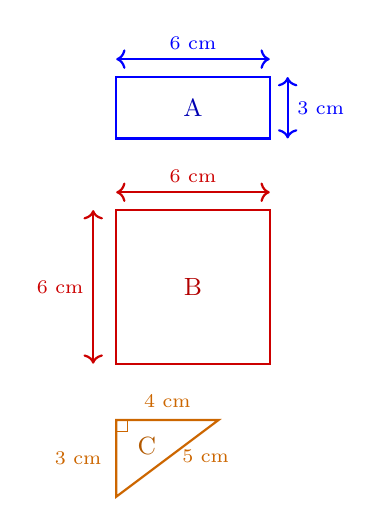
\begin{tikzpicture}[scale=0.65]

  %--- Shape A: Rectangle, 6 cm × 3 cm ---
  \draw[thick, blue] (0,9.5) rectangle (3,8.3);
  \draw[blue, thick, <->] (0,9.85) -- (3,9.85);
  \node[blue, above] at (1.5,9.85) {\scriptsize 6 cm};
  \draw[blue, thick, <->] (3.35,8.3) -- (3.35,9.5);
  \node[blue, right] at (3.35,8.9) {\scriptsize 3 cm};
  \node[blue!70!black] at (1.5,8.9) {\small A};

  %--- Shape B: Square, 6 cm × 6 cm ---
  \draw[thick, red!80!black] (0,6.9) rectangle (3,3.9);
  \draw[red!80!black, thick, <->] (0,7.25) -- (3,7.25);
  \node[red!80!black, above] at (1.5,7.25) {\scriptsize 6 cm};
  \draw[red!80!black, thick, <->] (-0.45,3.9) -- (-0.45,6.9);
  \node[red!80!black, left] at (-0.45,5.4) {\scriptsize 6 cm};
  \node[red!70!black] at (1.5,5.4) {\small B};

  %--- Shape C: Right-angled triangle, legs 4 cm and 3 cm, hypotenuse 5 cm ---
  % Vertices: right angle at (0,2.8), base to (2,2.8), height down to (0,1.3)
  \draw[thick, orange!80!black] (0,2.8) -- (2,2.8) -- (0,1.3) -- cycle;
  % Right angle mark at (0,2.8)
  \draw[orange!80!black] (0.22,2.8) -- (0.22,2.58) -- (0,2.58);
  % Labels
  \node[orange!80!black, above] at (1.0,2.85) {\scriptsize 4 cm};
  \node[orange!80!black, left] at (-0.1,2.05) {\scriptsize 3 cm};
  % Hypotenuse label: midpoint of (2,2.8)--(0,1.3) = (1, 2.05)21
  \node[orange!80!black, right] at (1.1,2.1) {\scriptsize 5 cm};
  \node[orange!70!black] at (0.6,2.3) {\small C};

\end{tikzpicture}
\end{center}

\column{0.62\textwidth}
\small
\begin{enumerate}
  \begin{multicols}{2}
    \item $6 \times 3 = \ ?$
    \item $\frac{3}{24} + \frac{5}{24} = \ ?$
  \end{multicols}
  \begin{multicols}{2}
    \item $\tfrac{1}{2} \times 4 \times 3 = \ ?$
    \item $-3 \times -2= \ ?$
  \end{multicols}
  \item Find the mean of $\ 8,\ 14,\ 20$.
  \item What fraction of $60$ is $6$?\quad Simplify fully.
\end{enumerate}
\vspace{-1.2em}
\begin{enumerate}
  \setcounter{enumi}{6}
  \item Find the \textbf{area} of each shape A, B and C.
  \item Find the \textbf{perimeter} of each shape A, B and C.
  \item Find the \textbf{mean area} of the three shapes.
  \item Find the \textbf{mean perimeter} of the three shapes.
  \item What fraction of the total area does shape C make up?
\end{enumerate}

\end{columns}
\end{frame}

%------------------------------------------------
% SLIDE 2: Areas, Perimeters, Mean & Fractions
%------------------------------------------------
\begin{frame}{Starter}

\vspace{-1em}

\begin{columns}

\column{0.38\textwidth}
\begin{center}
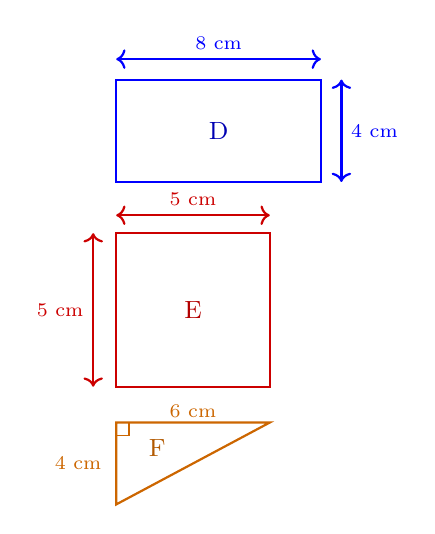
\begin{tikzpicture}[scale=0.65]

  %--- Shape D: Rectangle, 8 cm × 4 cm ---
  \draw[thick, blue] (0,9.5) rectangle (4,7.5);
  \draw[blue, thick, <->] (0,9.9) -- (4,9.9);
  \node[blue, above] at (2,9.9) {\scriptsize 8 cm};
  \draw[blue, thick, <->] (4.4,7.5) -- (4.4,9.5);
  \node[blue, right] at (4.4,8.5) {\scriptsize 4 cm};
  \node[blue!70!black] at (2,8.5) {\small D};

  %--- Shape E: Square, 5 cm × 5 cm ---
  \draw[thick, red!80!black] (0,6.5) rectangle (3,3.5);
  \draw[red!80!black, thick, <->] (0,6.85) -- (3,6.85);
  \node[red!80!black, above] at (1.5,6.85) {\scriptsize 5 cm};
  \draw[red!80!black, thick, <->] (-0.45,3.5) -- (-0.45,6.5);
  \node[red!80!black, left] at (-0.45,5) {\scriptsize 5 cm};
  \node[red!70!black] at (1.5,5) {\small E};

  %--- Shape F: Right-angled triangle, legs 6 cm and 4 cm ---
  \draw[thick, orange!80!black] (0,2.8) -- (3,2.8) -- (0,1.2) -- cycle;
  \draw[orange!80!black] (0.25,2.8) -- (0.25,2.55) -- (0,2.55);
  \node[orange!80!black, above] at (1.5,2.7) {\scriptsize 6 cm};
  \node[orange!80!black, left] at (-0.1,2.0) {\scriptsize 4 cm};
  \node[orange!70!black] at (0.8,2.3) {\small F};

\end{tikzpicture}
\end{center}

\column{0.62\textwidth}
\small
\begin{enumerate}
  \begin{multicols}{2}
    \item $8 \times 4 =\ ?$
    \item $\frac{7}{20} + \frac{9}{20} =\ ?$
  \end{multicols}
  \begin{multicols}{2}
    \item $\tfrac{1}{2} \times 6 \times 4 =\ ?$
    \item $-5 \times 4 =\ ?$
  \end{multicols}
  \item Find the mean of $\ 6,\ 12,\ 18$.
  \item What fraction of $80$ is $12$?\quad Simplify fully.
\end{enumerate}

\vspace{-1.2em}

\begin{enumerate}
  \setcounter{enumi}{6}
  \item Find the \textbf{area} of each shape D, E and F.
  \item Find the \textbf{perimeter} of each shape D, E and F.
  \item Find the \textbf{mean area} of the three shapes.
  \item Find the \textbf{mean perimeter} of the three shapes.
  \item What fraction of the total area does shape F make up?
\end{enumerate}

\end{columns}
\end{frame}

\end{document}